\documentclass[11pt,a4paper]{article}
\usepackage{a4wide}
\usepackage{natbib}
\usepackage{graphicx}
\usepackage{wrapfig}
\usepackage{amsfonts}

\usepackage{hyperref}
\usepackage{xcolor}
\usepackage[tikz]{bclogo}
\usepackage[framemethod=tikz]{mdframed}

\mdfdefinestyle{mystyle}{%
  rightline=true,
  innerleftmargin=10,
  innerrightmargin=10,
  outerlinewidth=3pt,
  topline=false,
  rightline=true,
  bottomline=false,
  skipabove=\topsep,
  skipbelow=\topsep
}

\setlength{\parindent}{0cm}

\begin{document}

\title{BSc Project Description\\\textbf{Learning to Play Tetris using
    the Covariance Matrix Adaptation
    Evolution Strategy}}
\date{\today}
\maketitle

% Removed because Motivation and background is the same
%\section{Background}


\subsection{Previous work \label{prevWork}}
Over the time, numerous researchers has tried different feature 
sets and applied various optimizers to find the best 
possible Tetris controllers. Researches in the field
of reinforcement learning have approached the task of learning Tetris
in various ways. Some have implemented exact versions of the original game
where the artificial Tetris player will have to interact with the 
game much like a human player. In these games the state of the board is not limited
to just the board configuration and the current piece, but also where in the 
board the piece is located. Hence, these controllers does not model actions 
as locations to drop the piece, but rather 'button presses' that controls the
fall of the piece. Yet, from the literature we have read, the most commonly applied 
type of controller is the one used in the MDPTetris platform. As mentioned earlier,
to create an efficient controller one can adjust two settings, namely the featureset 
and the associated weights. 
The specifics of how to tune the weighting is a topic that is 
explored along with finding the feature sets themselves. A common 
feature set, the Dellacherie feature set (see figure \ref{table:dellfeat}),
was originally tuned by hand with trial and error approach with a surprisingly 
good result. Yet, the most common approach is to apply some optimization 
algorithm to adjust the weighting.
The features used are typically
ones that attempt to mimic the board conditions that would
normally catch the attention of a human player, such as
how high the overall pile of pieces is and how many holes 
the board has. In \citep{scherrer2009:b} table 1, a table 
presents some feature sets used throughout various publications
on the subject. The feature sets applied in this thesis are 
Dellacherie and the Bertsekas feature sets 
(see figure \ref{table:dellfeat} and \ref{table:bertfeat}) due 
to their recurring usage across various articles.
Many authors have had success
with applying evolutionary stochastic search methods for tuning 
the weights of the feature sets towards
efficient controllers. However, the goal of most research 
is to outperform existing controllers and push the boundaries
of performance when learning Tetris. This means that the objective of
these researchers is often to craft feature sets that perceives the 
board in a way that allows the agent to make the best possible decisions.
Thus the focus in most works is combined on finding good feature sets and 
finding good ways to optimize the weights of the set. In this thesis,
our goal is not to find a controller that outperforms any existing one,
but rather to investigate the learning properties of the optimization algorithms.
For this purpose
we are in particular addressing the
Cross-Entropy method described in detail in \citep{cetut2014} and the
Covariance Matrix Adaption Evolution Strategy (CMA-ES), described 
in \citep{hansen2011}. The particular Cross-Entropy method applied 
is the one described in \citep{szita:06} as the "Noisy Cross Entropy Method".\\

\begin{figure}[h!]
\begin{center}
\begin{tabular}{| l | p{8cm} |}
\hline
\textbf{Feature} & \textbf{Description}\\
\hline
Landing height & The height of the last piece when it was placed\\
\hline
Eroded piece cells & Number of rows cleared in the last move
times the number of bricks cleared from the last move\\
\hline
Row transitions & Number of horizontal cell transitions\\
\hline
Column transitions & Number of vertical cell transitions \\
\hline
Holes & Number of empty cells covered by a full cell\\
\hline
Board wells & Cumulative sum of cells to the depth of
the board wells.\\
\hline
\end{tabular}
\end{center}
\caption{features of the Dellacherie featureset \label{table:dellfeat}}
\end{figure}

\begin{figure}[h!]
\begin{center}
\begin{tabular}{| l | p{8cm} |}
\hline
\textbf{Feature} & \textbf{Description}\\
\hline
Max height & Height height of the highest occupied block\\
\hline
Column height & Height of each column\\
\hline
Height difference & The height difference between columns\\
\hline
\end{tabular}
\end{center}
\caption{features of the Dellacherie featureset \label{table:bertfeat}}
\end{figure}


Currently, many researchers have proposed numerous 
feature sets and multiple 
optimization methods have been explored. 
The Dellacherie controller is very widely used across many resources
\citep{fahey}. This controller was hand-tuned by trial and error,
and did originally, on a regular non-simplified Tetris game, achieve an average of
660 000 lines. The same feature set (see figure \ref{table:dellfeat}) is 
often incoorporated in later works when optimizing controllers. An earlier
feature set is the set proposed by \citep{Bertsekas} referred to as Bertsekas and
Tsitsiklis features. In 2006, Szita and L\H{o}rincz \citep{szita:06} applied the Cross-Entropy
method using the Bertsekas and Tsitsiklis features. They report that using no noise,
their controller converged at 300 000 lines on average. 
The best result reported in \citep{szita:06}
is when decreasing noise is applied, 
in which the controller's score exceeded 800 000 lines. 
However, in a later paper, using Dellacherie, 
Bertsekas and two selfdefined features achieved 
35.000.000 lines $\pm 20\%$  \citep{scherrer2009}.\\




\input{Background/objectiveFunction}

\subsection{Optimizers \label{Optimizers}}

In this thesis, the Cross-Entropy method and the Covariance Matrix Evolution 
Strategy are compared. Both of the methods fall into the category of 
\textit{stochastic optimization}
methods. These methods are useful for 
optimization problems where the gradient is not available.
The optimization functions aim to optimize 
the parameter set $\textbf{\individual }$
for the objective function $\fitnessFunction$.
\begin{align}
\hat{\textbf{\individual }} &= 
arg \  \underset{\textbf{\individual }}{max} \  
\fitnessFunction (\textbf{\individual }) \ 
:\mathbb{R}^{\dimensions } \rightarrow \mathbb{R}
\end{align}

In these methods, the optimizing algorithm uses a family of parametric distributions,
and maintains a mean $\mean $ along with other parameters
to search the best possible solution for the objective function.  
In the case studied in this thesis
both the CMA-ES and Cross-entropy methods use a 
Gaussian distribution to sample solutions to the objective function.
Hence, both of the functions aim to find a mean 
$\mean $ and an $\dimensions \times \dimensions$ matrix 
$\varianceMatrix $\footnote{In \citep{hansen2011}, 
$\sigma$ is used for step-size in CMA-ES, so $\varianceMatrix $ is instead introduced
as an arbitrary $\dimensions \times \dimensions$ matrix in its place.}, such that when
a vector $\textbf{\individual }$ is sampled by 
$\textbf{\individual } \sim \mathcal{N}\left( \mean, \varianceMatrix \right)$, 
then $\fitnessFunction (\textbf{\individual })$ 
is likely to yield preferable results.\\
\\
The algorithms work iteratively, such that the mean and variance 
of the distribution 
is altered for each iteration $\generation $.
The algorithms start by initializing the 
parameters either at random or at some fixed point. A common 
configuration is setting the mean to 
all zeros and the standard deviation to the identity matrix.
Thus, for the first iteration $\generation = 0$, a configuration could be:
\begin{align}
\mean^{(0)} =
\begin{bmatrix}
0\\
\vdots\\
0
\end{bmatrix},\ \ 
\varianceMatrix^{(0)} = 
\begin{bmatrix}
1 & \hdots & 0\\
\vdots & \ddots & \vdots\\
0 & \hdots & 1
\end{bmatrix}
\end{align}

The superscript of $(0)$ notes that the values occur in iteration 0.\\
\\
In each iteration, the algorithms sample $\populationSize$ candidate solutions 
and evaluate their fitness
against the objective function. When each of the solutions are evaluated,
they are ordered according to their fitness:
\begin{align}
\{\textbf{\individual }_{1}, \hdots, 
\textbf{\individual }_{\populationSize }\}\ \ \text{Such that}\ \ 
\fitnessFunction(\textbf{x}_1) \geq 
\fitnessFunction(\textbf{\individual }_2), \hdots, 
\fitnessFunction(\textbf{\individual }_{\populationSize  - 1}) \geq 
\fitnessFunction(\textbf{\individual }_{\populationSize })
\end{align}

The mean and standard deviation for the next iteration, 
that is $m^{(\generation+1)}$ and $M^{(\generation+1)}$, are
then updated usually by considering the best of the ordered solutions. How exactly
these parameters are updated is individual for each method and can be seen in the following
sections.




\subsection{CE (Cross Entropy) \label{CrossEntropy}}
CE is described through many papers in 
slightly different ways. This section
describes the algorithm in a similar fashion 
to \citep{thiery:09}.\\
\\
This method uses a Gaussian distribution to 
sample sample vectors for the objective function
$\fitnessFunction$. The algorithm aims to 
adjust the parameters of the distribution
such that samples $\individual$ drawn from the distribution
gives the best possible results when applied to the
objective function $\fitnessFunction \left( \individual \right)$.\\
\\
The Cross-Entropy method starts with an initial 
mean $\mean$ which is an $n$-dimensional vector
typically set to 0
\begin{align}
\mean^{(0)} = \begin{pmatrix}
0\\
\vdots\\
0
\end{pmatrix} 
\end{align}

The second argument to the gaussian distribution is a 
diaginal matrix which contains the variance for each 
component

\begin{align}
\varianceMatrix^{(0)} =
\begin{bmatrix}
\sigma_1^{2} & \hdots & 0\\
\vdots & \ddots & \vdots\\
0 & \hdots & \sigma_{\dimensions}^{2}
\end{bmatrix}
\end{align}
The algorithm will in each generation sample a set of search points
and rank these using the objective function.
In each generation, $\populationSize$ vectors are sampled by 
$\individual_{i} \sim \mathcal{N} \left(\mean, \varianceMatrix^{2} \right)
,\ i \in \{1,\dots,\populationSize \}$. The vectors are all evaluated 
against the fitness function and ordered such that $\fitnessFunction \left( \individual_{1} \right) \geq, \dots, \geq \fitnessFunction \left( \individual_{\populationSize} \right)$
, and the $\offspringNumber$ best are chosen for updating the distribution 
parameters. The mean is updated as the centroid of the chosen vectors, and
the variance in each dimension is set to the variance of the chosen vectors in each 
dimension.\\

The pseudo code and details of the algorithm can be seen in figure
\ref{fig:ceCode} on page \pageref{fig:ceCode}.

\begin{figure}[H]
\hrule
\vspace{0.2cm}
{\centering  \textit{Noisy cross-entropy method}}
\vspace{0.2cm}
\hrule
\begin{algorithmic}
\State{\textbf{input}}
\State{$\fitnessFunction$ : The function that estimates the performance of a vector $\individual$}
\State{($\mean^{(0)}$, $\varianceMatrix^{(0)}$): The mean and variance of the initial distribution}
\State{$\populationSize$ : The number of vectors sampled per generation/iteration}
\State{$\offspringNumber$: The number of offspring selected for the new mean}
\State{$\noise_{\generation}$: The noise added to each generation/iteration}
\\

\Loop
\State{Generate $\populationSize$ vectors $\individual_{1}, \individual_{2}, \dots, \individual_{\populationSize}$ from $\mathcal{N}(\mean^{(\generation)}, \varianceMatrix^{(\generation)})$}
\State{Evaluate each vector using $\fitnessFunction$}
\State{Select the $\offspringNumber$ vectors with the highest evaluation}
\State{Update $\mean^{(\generation + 1)}$ based on the $\offspringNumber$ best vectors}
\State{Update $\varianceMatrix^{(\generation + 1)}$ based on the $\offspringNumber$ best vectors + $\noise^{(\generation)}$}
\EndLoop
\end{algorithmic}
\hrule
\caption{The pseudo code for the Cross-Entropy algorithm \label{fig:ceCode}}
\end{figure}

\subsubsection{Input}

\textbf{The objective function \label{CEObjective}} \\
The objective function $\fitnessFunction$ is a 
function used to rank the value of a sampled vector.
As described in the 'Optimizers' section, CE is a general stochastic 
iterative algorithm that tries to solve an optimization problem of 
the form \citep{thiery:09}:
\begin{align}
\hat{\textbf{\individual }} &= 
arg \  \underset{\textbf{\individual }}{max} \  
\fitnessFunction (\textbf{\individual }) \ 
\end{align}
Where $x$ corresponds to a given vector, 
and $\fitnessFunction$ is our actual objective function. 
\\

\textbf{The mean and variance of the gaussian distribution} \\
Here $\mean^{(\generation)}$ is the mean and  
$\varianceMatrix^{(\generation)}$ is the covariance matrix, with 
the variance in each dimension along the diagonal, and zeros elsewhere. 
The parameters in the Gaussian distribution are ($\mean^{(\generation)}$,
$\varianceMatrix^{(\generation)}$). 
More specifically this Gaussian distribution is defined as 
\begin{align}
\mathcal{N}(\mean^{(\generation)},\varianceMatrix^{(\generation)})
\end{align}

Where $\generation$ denotes the current iteration.\\


\textbf{The number of vectors}\\
$\populationSize$ is the number of vectors sampled in each generation.
\\

\textbf{The number of selected vectors / parents}\\
$\offspringNumber$ is the number of vectors which are selected to compute 
the new mean $\mean_{\generation + 1}$, and variance
$\varianceMatrix^2_{\generation + 1}$, for next generation/iteration. 
These offspring vectors gets selected 
directly by taking the $\offspringNumber$ best ranked
vectors.
\\

\textbf{The noise term}\\
The noise factor, $\noise_{\generation}$, 
is the amount of noise which 
is applied to the variance $\varianceMatrix^2$ in
iteration/generation 
$\generation$. In general, noise is used to prevent
the algorithm from 
getting narrowing down to an undesired local optimum, but
rather explore new solutions.
The noise term can be any
function of $\generation$. Among 
the most described noise types are: no noise, constant noise 
and linear decreasing noise \citep{szita:06}. 
When using no noise, $\noise_{\generation}$ 
is simply set to zero. When using constant noise, 
the same value is 
added to the variance $\varianceMatrix^2$ 
in each iteration/generation. 
When using linear decreasing noise, 
$\noise_{\generation}$ is often set as
$\noise_{\generation}=max(5- \generation /10,0)$.
\\

\subsubsection{Loop}

\textbf{Sampling the population}\\
The first step of the loop is to generate the new generation 
consisting of $\populationSize$ vectors. 
These vectors are drawn from the distribution 
$\individual_{i}\sim \mathcal{N}(\mean_{\generation},\varianceMatrix^2_{\generation})$.
\\

\textbf{Evaluating the population}\\
After sampling the population, the algorithm needs to order the vectors to find the $\offspringNumber$ best vectors, each vector $\individual_{i}\ ,\ i \in \{1, \dots, \populationSize\}$ is evaluated using $\fitnessFunction$. 
The value from the objective function then yields 
the estimated performance of each individual.
\\

\textbf{Selecting the parents}\\
As each $\individual_{i}$ has an assigned evaluation value, and the 
$\offspringNumber$ best vectors gets selected by 
taking the $\individual_{i}$ vectors with the highest ranking.
\\

\textbf{Updating the distribution parameters}\\
When updating the distribution parameters for the next iteration
($\mean^{(\generation + 1)}$,$\varianceMatrix^{(\generation + 1)}$), 
the mean is updated by computing the centroid of the 
$\offspringNumber$ highest ranking vectors. This is formally defined as:
\begin{align}
\mean^{(\generation +1)}:=\frac{\sum_{i=1}^{\offspringNumber} \individual_{i}}{\offspringNumber}
\ \ \ 
\text{where}
\ \ \ 
\fitnessFunction \left( \individual_{1} \right) \geq, \dots, 
\geq \fitnessFunction \left( \individual_{\offspringNumber} \right) \geq, 
\dots, \geq \fitnessFunction \left( \individual_{\populationSize} \right)
\end{align}
The diagonal matrix of variances $\varianceMatrix^{(\generation + 1)}$ is updated 
to match the variance of the $\offspringNumber$ best
vectors, such that the variance in dimension $k$ 
matches the variance of the $\offspringNumber$
in dimension $k$. Hence, for $k \in \{ 1,\dots,\dimensions \}$,
the $(k,k)$'th entry in the variance matrix is 
updated 
This is formally defined as:
\begin{align}
{\varianceMatrix^{(\generation +1)}}_{k,k}:=\frac{\sum_{i}^{\offspringNumber}
({\individual_{i}}_k - \mean_{\generation +1})^2}{\offspringNumber} + 
\noise_{\generation + 1}\ ,\ \ k \in \{ 1,\dots,\dimensions \}
\end{align}

\subsection{CMA-ES \label{CMAtheory}}


This description is based on the tutorial written by Nikolaus Hansen
\citep{hansen2011}. This section will not focus on the theoretical derivation
of CMA, but rather how it deviates from Cross Entropy. 
The CMA operates on a general level much like the Cross Entropy 
method, but includes some features that increases the adaptability 
of the algorithm.\\
\\
The CMA, like the Cross Entropy, uses a Gaussian distribution to
search for good solutions to $\fitnessFunction$. Yet, for the 
variance parameter, the CMA provides a full covariance matrix.
As the Cross Entropy method only provides a diagonal matrix of scalers,
it's restricted to only scaling the ellipsoid of equal density along
the coordinate axes. The CMA however, with a full covariance matrix,
allows the ellipsoid to rotate arbitrarily in the search space.\\
Another difference between the two algorithms is that 
Cross Entropy only considers the next population when updating the
distribution parameters, while the CMA keeps track of 
some information from earlier 
generations. This allows the CMA somewhat keep track of the evolution 
of the sampled vectors.\\
The CMA also differs from Cross Entropy in how it evaluates the influence 
of the parent vectors. As Cross Entropy weights all vectors equally when 
moving the mean. The CMA, at least from the implementation in SHARK, 
has the option of taking a weighted combination of the offspring in order
to bias towards the better vectors.

\begin{figure}[H]
\hrule
\vspace{0.2cm}
{\centering  \textit{CMA-ES}}
\vspace{0.2cm}
\hrule
\begin{algorithmic}
\State{\textbf{input}}
\State{$\fitnessFunction$: The function that estimates the performance of a vector $\individual$}
\State{($\mean$, $C$): The mean and variance of the initial distribution, where 
$C$ is the covariance matrix usually set to $C=I$}
\State{$\lambda$: The number of vectors sampled per generation/iteration}
\State{$\offspringNumber$: The number of offspring selected for the new mean}
\\
\State{\textbf{initialization}}
\State{Set initial internal parameters}
\\
\Loop
\State{Increment generation counter2}
\State{Sample new generation}
\State{Evaluate each vector using $\fitnessFunction$ and recombine}
\State{Covariance matrix adaption}
\State{Step-size control}
\EndLoop
\end{algorithmic}
\hrule
\caption{The pseudo code for the Cross-Entropy algorithm \label{fig:cmaCode}}
\end{figure}

Note here that the population size in this section is denoted as
$\lambda$ as opposed to $\populationSize$. Also the iteration/generation 
counter is referred to s $g$ rather than $\generation$. 
This is to remain consistent 
with the tutorial.

\subsubsection{Input}

\textbf{The objective function} \\
This serves the same purpose as in Cross Entropy (see page \pageref{CEObjective}).
\\

\textbf{The mean and variance of the gaussian distribution} \\
Here $\mean^{(g)}$ is the mean and  
${C^{(g)}}^{2}$ is the variance 
of the gaussian distribution ($\mean^{(g)}$,
${C^{(g)}}^2$). 
More specifically this gaussian distribution is defined as 
\begin{align*}
\mathcal{N}(\mean_{\generation},\sigma C^2_{\generation})
\end{align*}

Where $g$ denotes the current iteration/generation.\\


\textbf{The number of vectors}\\
$\populationSize$ is the number of vectors sampled in each generation.
\\

\textbf{The number of offspring}\\
$\offspringNumber$ is the number of vectors which are used to compute 
the new mean very much like in Cross Entropy. However the CMA algorithm
is not bound to weight each vec tor equally. It has the option to assign 
a weight to each vector and hence biasing towards the better solutions.
\\


\subsubsection{Initialization}


Set parameters
\begin{align}
\lambda, \offspringNumber, w_{i \dots \offspringNumber}, c_{\sigma}, d_{\sigma}, c_c, c_1, c_{\offspringNumber}
\end{align}
To their default values according to table 1 in \citep{hansen2011}.

Set evolution path $p_{\sigma} = 0$, $p_{c} = 0$, covariance matrix $C = I$ and $g = 0$

Where:

\begin{align}
\lambda, \mu, g &\in \mathbb{N}\\
w_i,\dots,w_{\mu}, c_{\sigma}, d_{\sigma}, c_c, c_1, c_{\lambda}, &\in \mathbb{R}\\
p_{c}, p_{\sigma} &\in \mathbb{R}^{\dimensions}\\
C &\in \mathbb{R}^{\dimensions \times \dimensions}
\end{align}

Again, note that $\lambda$ has the meaning of $\populationSize$ from earlier, that
is $\lambda$ is in this case the population size. $\mu$ however, is still the number
of vectors that contribute to the updating of distribution parameters, namely the 
parent size.\\
\\
In this algorithm, the distribution used is multivariate normal distribution defined
as 
\begin{align}
\mathcal{N} \left( m,  \sigma^2 C \right)
\end{align}
This distribution describes the set of correlated real-valued vectors that
clusters around the mean vector $m$ and has a covariance described by the
matrix $C$. The covariance matrix describes the 'shape' of the space in which 
the vectors are most likely to be sampled. For illustrative purposes,
the shape of the sampling space is drawn as an ellipseoid.
This ellipoid depicts a set of points that has equal denity 
in the probability denisty function of $C$, and is hence refered to 
as the ellipse of equal density.
With a covariance matrix $C$
the ellipsoid is defined as points that stisfies
$\{x \in R^{\dimensions} | x^{T} C^{-1} x = 1\}$.
When illustrating this, the step-size is set as $\sigma = 1$ for simplicity.\\
\\
The matrix $C^{-1}$ is decomposed as $C^{-1} = B D^{-2} B^T$, where $B$ is a rotation 
matrix that rotates from the coordinate axises into the principal axises of $C$, and 
$D^{-2}$ is the diagonal matrix 
$\text{diag} \left( \frac{1}{d_{1}^2},\dots, \frac{1}{d_{\dimensions}^2} \right)$
where $d_{i}$ is the $i$'th eigenvalue of $C$. Figure \ref{fig:ellipse} shows an example
of how to determine if a point lies on the ellipsoid. In this example, the aim is to 
determine if the point $x$ lies on the two-dimensional ellipsoid, hence checking if 
$x^{T} C^{-1} x = 1 \Leftrightarrow x^{T} B D^{-2} B^T x = 1 $ holds. In figure 
\ref{fig:ellipse}, $l$ is the length from the origin of the ellipse to the edge.
Consider the operation
\begin{align}
B D^{-2} B^T x \label{eq:rotscal}
\end{align}

The order of operations are the following. 
$B^{T}$ rotates $x$ from the principal axises of $C$
into the coordinate axises. Then $D^{-2}$ scales the point by $\frac{1}{l^2}$ where
$l$ is the length from the ellipsoid origin to the edge. Finally, $B$ rotates the point 
back in the original direction. thus, (\ref{eq:rotscal}) has the same effect as
\begin{align}
\frac{1}{l^2} x
\end{align}
Hence, the entire operation is equivalent to
\begin{align}
x^{T} B D^{-2} B^T x &= x^{T} \frac{1}{l^2} x = \frac{1}{l^2} x^{T} x
= \frac{1}{l^2} ||x||^2
\end{align}
This means that if $||x||^2 = l^2$ then $x$ lies on the ellipse.
In the example of figure \ref{fig:ellipse}, $x$ is not 
on the ellipse.


\begin{figure}[H]
\begin{center}

\end{center}
\begin{center}
\ellipseFigure
\end{center}
\caption{Illustration of $\{x \in R^{\dimensions} | x^{T} C^{-1} x \stackrel{?}{=} 1\}$ \label{fig:ellipse}}
\end{figure}

\subsubsection{Loop}

\textbf{Increment iteration counter}

If the stopping criteria is not met
\begin{align}
g &= g+1
\end{align}
Otherwise, stop.\\


\textbf{Sample new generation}\\
Sample new population of search points, for $k = 1, \dots, \lambda$.
The aim is to sample vectors in the following form
\begin{align}
\individual_{k} \sim \mathcal{N}(m, \sigma^2 C)
\end{align}


To generate the sample for the generation, the covariance matrix is first 
decomposed using principal component analysis into
\begin{align}
C = B D^2 B^{T}
\end{align}

Where $B = \begin{bmatrix}
b_1, & \dots, & b_\dimensions
\end{bmatrix}$ 
is am orthogonal basis of eigenvectors, and  
$D = \text{diag}\left(d_1, \dots, d_\dimensions\right)$
is a diagonal matrix that contains all eigenvalues of $C$.\\
\\
Intermediately, the vectors are sampled from a Gaussian distribution 
with zero mean and
the identity matrix as variance.
\begin{align}
z_{k} &\sim \mathcal{N}(0, I)
\end{align}

$z_k$ is then multiplied by a factor that causes the them to form 
after the covariance matrix $C$. From Hansens tutorial, it's derived that
\begin{align}
C^{-1} &= B D^{-2} B^{T}\\
C^{\frac{1}{2}} &= B D B^{T}
\end{align}

Thus, to get the effect of the covariance matrix to apply to the $z_k$
samples, the following is used

\begin{align}
\mathcal{N}\left( 0, C \right) \sim C^{\frac{1}{2}} \mathcal{N}\left( 0, I \right)
\end{align}

\begin{align}
y_{k} &= B D \underbrace{B^{T} z_{k}}_{\sim \mathcal{N}(0, I)} \sim \mathcal{N}(0, C)\\
y_{k} &= B Dz_{k} \sim \mathcal{N}(0, C) \label{eq:sampley}
\end{align}

$B$ is the orthogonal basis of vectors of unit length, which means that 
$B$ is purely a rotation matrix. Due to this, $B^{T} z_{k}$ only rotates
$z_k$ yielding the same distribution. After this, the $BD$ is multiplied,
which applies the scale such that each vector is scaled to match the
variance in the principal axises of the covariance matrix, and $B$ 
will rotate each sample such that it aligns with the principal axises
of $C$. After this step, $y_{k}$ now resemble the vectors that rotated and scaled
to match shape of the covariance matrix.\\

The mean and step-size $\sigma$ is applied.
\begin{align}
x_{k} &= m + \sigma y_{k} \sim \mathcal{N}(m, \sigma^2 C) \label{eq:finalSample}
\end{align}



Finally, the $x_{k}$ vector resemble a realization of the Gaussian distribution
with mean $m$ and covariance matrix $C$ scaled by the step-size $\sigma$.
Am illustration of the sampling process in two dimensions can be seen in figure \ref{fig:sampleing} where 
\begin{align}
\sigma = 1,\ B = \begin{bmatrix}
{b_1}_x & {b_2}_x\\
{b_1}_y & {b_2}_y
\end{bmatrix},\ D = \begin{bmatrix}
d_1 & 0\\
0   & d_2
\end{bmatrix}
\end{align}


\begin{figure}[H]
\begin{center}
\begin{tabular}{c c c}
\begin{tikzpicture}[scale=0.5]
\draw [->] (0,-5) -- (0,5);
\draw [->] (-5,0) -- (5,0);
\node at (0,0) {};
\draw  (0,0) ellipse (2 and 2);
\draw (0,0) -- (2,0);
\draw [decorate,decoration={brace,amplitude=5,raise=2},yshift=0pt]
(0,0) -- (2,0) node [black,midway,xshift=0,yshift=15] {1};
\end{tikzpicture} &
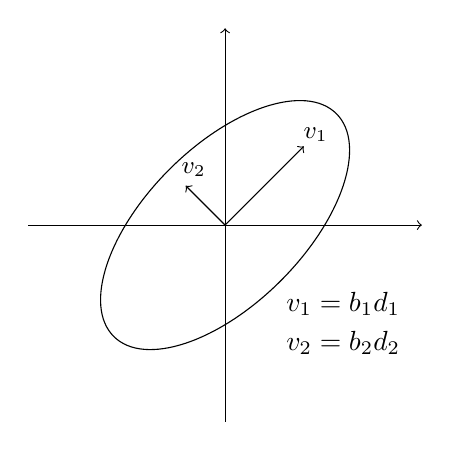
\begin{tikzpicture}[scale=0.5]
\draw [->] (0,-5) -- (0,5);
\draw [->] (-5,0) -- (5,0);
\node at (0,0) {};
\draw [rotate=45] (0,0) node (v1) {} ellipse (4 and 2);
\draw [->] (0,0) --  (2,2);
\draw [->] (0,0) -- (-1,1);
\node at (-0.8,1.4) {\small $v_2$};
\node at (2.3,2.3) {\small $v_1$};
\node at (3,-2) {$v_1 = b_1 d_1$};
\node at (3,-3) {$v_2 = b_2 d_2$};
\end{tikzpicture} &
\begin{tikzpicture}[scale=0.5]
\draw [->] (0,-5) -- (0,5);
\draw [->] (-5,0) -- (5,0);
\node at (1,1) {};
\draw [rotate=45] (1.5,0) node (v1) {} ellipse (4 and 2);
\draw [->](1,1) -- (3,3);
\draw [->] (1,1) -- (0,2);
\draw [fill] (1,1) ellipse (0.1 and 0.1);
\node at (2,1) {\small $m$};
\end{tikzpicture}\\
$z_{k} \sim \mathcal{N}(0, I)$ & $y_{k} \sim B Dz_{k}$ & $x_{k} \sim m + \sigma y_{k} \sim \mathcal{N}(m, \sigma^2 C)$
\end{tabular}
\end{center}
\caption{The steps of the sampling process \label{fig:sampleing}}
\end{figure}


\textbf{Evaluate each vector using $\fitnessFunction$ and recombine}\\
As each vector is evaluated, they are ranked such that
$\fitnessFunction{ \left( \individual_{i} \right) } \geq \dots \geq \fitnessFunction{ \left( \individual_{\offspringNumber} \right)} \geq \dots \geq \fitnessFunction{ \left( \individual_{\lambda} \right)}$.

\begin{align}
\langle y \rangle_{w} &= \sum^{\offspringNumber}_{i = 1}w_{i} y_{i : \lambda}
\end{align}

Where the notion of $y_{i : \lambda}$ means the $i$'th element in ranked list of vectors
where $y_1$ is the best ranked vector.

\begin{align}
\sum^{\offspringNumber}_{i = 1} w_{i} = 1, w_{i} > 0
\end{align}

$\langle y \rangle_{w}$ is a measure of a 'weighted center of mass',
and is part of the selection mechanism. The idea is to allow the selected vectors
to contribute differently to the update, and hence emphasize the higher 
ranking vectors. The individual weights are as the following

\begin{align}
w_i &= \frac{w_{i}'}{\sum^{\offspringNumber}_{j=1} w_j }
\end{align}

Where the $w_i'$ is used for a intermediate weighting value for the vectors.\\
In the Shark library, three built-in weighting types are implemented, each with
a distinct intermediate weight.

\begin{align}
\text{Equal}: &\quad w_i' = 1 \label{eq:recomType}\\
\text{Linear}: &\quad  w_i' = \offspringNumber - i\\
\text{Superlinear:} &\quad w_i' = ln \left( \offspringNumber + \frac{1}{2} \right)
- ln \left( i \right)
\end{align}
Thus, with the equal, each vector contributes equally, and with the other two, the 
higher ranking vectors has more influence on location of the 'center of mass' of 
the selection.

The new mean is computed as
\begin{align}
m^{(g+1)} &= m^{(g)} + \sigma \langle y \rangle_{w} = \sum^{\offspringNumber}_{i = 1} w_{i}x_{i:\lambda} \label{eq:movemean}
\end{align}
Such that the mean moves towards the 'center of mass' scaled by the step-size.
The details of step-size $\sigma$ is covered later in this section,
however in brief terms the step-size is meant to scale movements 
of the mean and the distribution area.\\
\\
In relation to the selection mechanism, the value $\mu_{eff}$ is introduced.
This is defined as
\begin{align}
\meff = \left( \sum_{i=1}^{\offspringNumber} w_i^2 \right)^{-1}
\end{align}
Hence $1 \leq \meff \leq \mu$. As an example, for the equal recombination
type, $\meff = \left( \sum_{i=1}^{\offspringNumber} w_i^2 \right)^{-1} = 1^{-1} =1$
In the tutorial by N. Hansen, it's mentioned that $\meff \approx 
\frac{\lambda}{4}$ indicates a good setting of $w_i$. The $\meff$ is 
measure of how much of the parent mass is used, and serves as a normalization 
factor in later equations.\\

\textbf{Covariance matrix adaption}

The idea of using the covariance matrix is to make new samples
resemble the covariance of the previous well-performing vectors, as opposed 
to the Cross Entropy algorithm that does not maintain any information of
previous samples.\\
\\
A evolution path of the movement of the means is introduced as $p_{c}$. This 
is a vector that holds the direction in which the mean has been moved in 
both the current generation, and in previous generations in 
a 'low-pass filter' like manner. Using the 
evolution path, the covariance matrix can take a shape that 
makes samples more likely to appear in the direction of successive 
movements of the mean.
The evolution path for generation $g+1$ is updated as

\begin{align}
p_{c}^{(g+1)} &= \underbrace{\left( 1 - c_{c} \right) 
p_{c}^{(g)}}_{\makebox[0pt]{\text{previous steps}}}  + 
\overbrace{h_{\sigma}}^{\makebox[0pt]{\text{{indicator function}}}}
\underbrace{\sqrt{c_{c} \left( 2 - c_{c} \right) \offspringNumber_{\text{eff}}}}_{
\makebox[0pt]{\text{normalization}}
}
\langle y \rangle_{w} \label{eq:epathc}
\end{align}
In (\ref{eq:epathc}), the term $\left( 1 - c_{c} \right) p_{c}^{(g)}$ makes 
the evolution path become influenced by earlier path steps. The learning rate
$c_c \in [0;1] $ indicates how much of the previous path is taken into account.
if $c_c = 0$, the previous path is not considered at all, and if $c_c = 1$ the path 
will only consist of the previous step. According to the tutorial, this is set
$c_c = \frac{4 + \mu_{eff} / \dimensions}{\dimensions + 4 + 2 \mu_{eff} / \dimensions}$.\\
\\
Th indicator function $h_{\sigma}$ is discussed in detail in the tutorial \citep{hansen2011}.
However, the main idea of this indicator function is.
\begin{align}
h_{\sigma}
\begin{cases} 1\ \ \ \text{if $||p_{\sigma}||$ is large} \\
              0\ \ \ \text{otherwise} %
\end{cases}
\end{align}
The purpose of this is to stall updating the evolution path when 
the length of the step-size evolution path becomes too large. The step-size
evolution path is covered in \textit{Step-size control}.\\
\\
The normalization factor 
$\sqrt{c_{c} \left( 2 - c_{c} \right) \offspringNumber_{\text{eff}}}$ is chosen such that
$p^{(g+1)}_{c} \sim \mathcal{N}\left(0, C \right)$ if $p_c^{(g)} \sim \mathcal{N} 
\left(0, C\right)$\\
To see that this holds, note that
\begin{align}
\langle y \rangle_{w} &= \frac{m^{(g+1)} - m^{(g)}}{\sigma}
\sim \frac{1}{\sqrt{\meff}}  \mathcal{N}\left(0, C \right)
\end{align}
\\
Thus, with the indicator function set aside
\begin{align}
p_{c}^{(g+1)} &\sim \left( 1 - c_{c} \right) 
\mathcal{N}\left(0, C \right) + 
\sqrt{c_{c} \left( 2 - c_{c} \right) \offspringNumber_{\text{eff}}}
\frac{1}{\sqrt{\meff}}\mathcal{N}\left(0, C \right) \label{eq:nomalization_start}\\
&\sim
\mathcal{N}\left(0, \left( 1 - c_{c} \right)^2 C \right) + 
\mathcal{N}\left(0, c_{c} \left( 2 - c_{c} \right)  C \right)\\
&\sim
\mathcal{N}\left(0, \left( 1 - c_{c} \right)^2 C + c_{c} \left( 2 - c_{c} \right)  C  \right)\\
&\sim \mathcal{N}\left( 0, C \right) \label{eq:nomalization_end}
\end{align}
Hance, the evolution path ios updated unbiased udner random selection.
\\
The covariance matrix is updated as follows
\begin{align}
C^{(g+1)} &= 
\underbrace{\left( 1 - c_{1} - c_{\offspringNumber} \right)C^{(g)}}_{
\makebox[0pt]{\text{{smoothing of previous steps}}}
} + 
\overbrace{c_{1} \left( p_{c}^{(g+1)} {p_{c}^{(g+1)}}^{T}\right)}^{
\makebox[0pt]{\text{{Rank-one update}}}
} +
\underbrace{c_{\offspringNumber} \sum^{\offspringNumber}_{i = 1} w_{i} y_{i : \offspringNumber} y_{i : \offspringNumber} ^{T}}_{
\makebox[0pt]{\text{{Rank-$\mu$ update}}}
} \label{eq:fullCMA}
\end{align}

Again, the first term is the smoothing of the previous covariance matrices.
the constants $c_1$ and $c_\mu$ are the learning rates for respectively the two
different updates, and the sum of them must not exceed 1, $c_1 + c_\mu \leq 1$.\\
\\
The rank-one update is meant to form the covariance matrix in a way such that 
it becomes more likely for the distribution to draw vectors in the direction of
successive steps. The term $c_{1} \left( p_{c}^{(g+1)} {p_{c}^{(g+1)}}^{T}\right)$
is first of all factored by the leaning rate $c_1$. The matrix computed as 
$p_{c}^{(g+1)} {p_{c}^{(g+1)}}^{T}$ is the outer product of the evolution path. 
Remember here that the $p_{c}^{(g+1)}$ is the smoothed vector that indicates 
the path in which the mean has been moved. Hence, the covariance will for this 
single vector be purely in the direction of the mean's movement. Also, as it's 
the outer product of just one vector, the rank of this matrix is one, hence the
name 'rank-one update'.\\
\\
The last term in (\ref{eq:fullCMA}) namely the rank-$\mu$ update
\begin{align}
c_{\offspringNumber} \sum^{\offspringNumber}_{i = 1} w_{i} y_{i : \offspringNumber} y_{i : \offspringNumber} ^{T} \label{eq:rankmuupdate}
\end{align}
Again, the entire term is factored by the learning rate $c_\mu$. The sum
of outer products yields and estimate for the covariance matrix of the vectors
sampled as $y_{i : \offspringNumber} \sim \mathcal{N}\left(0, C^{(g)}\right)$ 
(see (\ref{eq:sampley})). Thus (\ref{eq:rankmuupdate}) corresponds to the 
estimated covariance of the best selected vectors, with a weighting factor
such that the covariance of the highest ranking vectors may contribute the most.
The rank of the matrix in \ref{eq:rankmuupdate} is $min(\mu, \dimensions)$.\\
\\
As a result of this, when the covariance matrix is updated as in (\ref{eq:fullCMA})
the next sample will be more likely to be realized somewhat like the previous 
samples, somewhat in the direction in which the mean was moved and somewhat 
according to the covariance of the highest ranking vectors.
\\



\textbf{Step-size control}

In the CMA-ES algorithm, the step-size $\sigma$ is used as an isotropic scale across
each of the principal axis in the covariance matrix. Hence the stepsize is used as 
an 'overall' scaling mechanism when drawing vectors. The step-size is used when 
sampling the vectors in (\ref{eq:finalSample}) where it expands the variance 
of the distribution. When moving the mean in (\ref{eq:movemean}), the weighted 
selection mass \textbf{scaled} with the step-size is added to the mean.

\comment{PUT fig here}

First we consider the evolution path of the step-size $p_\sigma$ which is
updated a s follows.

\begin{align}
p_{\sigma}^{(g+1)} &= 
\underbrace{\left( 1 - c_{\sigma} \right) p_{\sigma}^{(g)}}_{
\makebox[0pt]{\text{{smoothing of previous steps}}}
}
+ 
\overbrace{\sqrt{c_{\sigma} \left( 2 - c_{\sigma} \right) \meff}}
^{
\makebox[0pt]{\text{{normalization}}}
} 
\underbrace{C^{- \frac{1}{2}}}_{
\makebox[0pt]{\text{{scale/rotation}}}
}
\langle y \rangle_{w}
\end{align}
The first term is the smoothing step as seen before only using the learning rate 
associated with the step-size evolution path but is similar to what is seen in
(\ref{eq:epathc}). The normalization constant is also very similar to the
equivalent factor in (\ref{eq:epathc}).\\
\\
A newly introduced factor is the $C^{-\frac{1}{2}}$ with the decomposition
$C^{-\frac{1}{2}} = B D^{-1} B^{T}$ which has the following effects. $B^{T}$
rotates the principal axises to align with the coordinate axises. 
$D^{-1}$ scales the axises into equal size, and finally, $B$ rotates the 
axises back into the original direction. The transform $C^{-\frac{1}{2}}$
has the effect of making the length of the $p_\sigma$ independent of 
direction as each dimension is normalized.\\
\\
The final effect is that
\begin{align}
p_\sigma^{(g+1)} &\sim \mathcal{N}\left(0, I \right)\\
\text{When }
p_\sigma^{(g)} &\sim \mathcal{N} \left(0, I \right)
\end{align}
With almost the same steps as (\ref{eq:nomalization_start}) through 
(\ref{eq:nomalization_end}).
\begin{align}
p_\sigma^{(g+1)} &\sim (1 - c_\sigma) \mathcal{N}\left( 0, I \right) + \sqrt{c_\sigma 
\left( 2-c_\sigma \right)\meff } {C^{(g)}}^{-\frac{1}{2}} \frac{1}{\sqrt{\meff}}
\mathcal{N} \left( 0, C^{(g)} \right)\\
&\sim \mathcal{N} 
\left( 
  0, 
  \left(  
    \left( 
      1-c_\sigma 
    \right)^2 + \sqrt{c_\sigma 
    \left(  
      2 - c_\sigma
    \right)}^2
  \right) I
\right) \sim \mathcal{N} \left( 0, I \right)
\end{align}

Hence, under random selection, the evolution path $p_\sigma \sim \mathcal{N} 
\left( 0, I \right)$.  The step-size is adapted by comparing the length
if the evolution path $||p_\sigma||$ with the expected length of a vector 
drawn from $\mathcal{N} \left( 0, I \right)$, that is
$\mathbb{E}||\mathcal{N}\left(0, I\right)||$. where 
$\mathbb{E}||\mathcal{N}\left(0, I\right)|| \approx \sqrt{n} + \mathcal{O}\left(1/n\right)$
The cases if this comparison are:

\begin{align}
\textbf{a: } ||p_\sigma^{(g+1)}|| &> \mathbb{E}||\mathcal{N}\left(0, I\right)|| 
\label{case1}\\
\textbf{b: } ||p_\sigma^{(g+1)}|| &< \mathbb{E}||\mathcal{N}\left(0, I\right)||
\label{case2}\\
\textbf{c: } ||p_\sigma^{(g+1)}|| &= \mathbb{E}||\mathcal{N}\left(0, I\right)||\label{case3}
\end{align}
In case \textbf{a} the steps are correlated and the idea is that a larger step-size
would cause the mean to move towards a desired location faster. In case \textbf{b},
the path is short and/or anti correlated. This means that the algorithm would benefit from
shorter steps, and therefore decrease the step-size. In the final case \textbf{c}, the 
steps appear perpendicular and the step-size appears reasonable.\\
\\
Eventually, the step-size is updated by the following.
\begin{align}
\sigma^{(g+1)} &= \sigma^{(g)} \cdot exp \left( \frac{c_{\sigma}}{d_{\sigma}} \left( \frac{||p_\sigma^{(g+1)}||}{E|| \mathcal{N}(0, I) ||} - 1 \right) \right)
\end{align}
Where $0 \leq \frac{c_\sigma}{d_\sigma} \leq 1$ is a damping factor for step-size changes.
This update of the step-size will scale the step-size unbiased in direction 
according to the cases in 
(\ref{case1}), (\ref{case2}) and (\ref{case3}).











\subsection{Normalization of samples \label{normalSamples}}
As mentioned in \citep{boumaza2009}, the vector that
describes the agent can very well be normalized such that the vector
is a point that lies on the $\dimensions$-dimensional hypersphere.\\
\\
The reason for this lies in the nature of the evaluation function.
When the controller chooses an action, it will evaluate all the
actions possible with the current piece. It will use the 
value function $\valueFunction$ of each state $\gameState_i$ and 
choose the state with the highest value from the value function.
Thus, if the states are ordered such that
\begin{align}
\valueFunction \left(  \gameState_1 \right) 
> \dots 
> \valueFunction \left( \gameState_\populationSize \right)
\end{align}

The agent then chooses the action that transitions from the current state 
to state $\gameState_1$.\\
Since the value function assess the state by the following
\begin{align}
\valueFunction (\gameState ) &= 
\sum_{i=1}^{\dimensions} \weight _{i}\feature _{i}(\gameState )
\end{align}

Then scaling the input of the agent, the weight vector $\weight$, by a
number $a \in \mathbb{R}, \ a > 0$ the assessment is changed by
\begin{align}
\sum_{i=1}^{\dimensions} a \weight _{i}\feature _{i}(\gameState ) &= 
a\sum_{i=1}^{\dimensions} \weight _{i}\feature _{i}(\gameState )\\
&= a \valueFunction \left( \gameState \right)
\end{align}

And the ordering remains
\begin{align}
a \valueFunction \left(  \gameState_1 \right) 
> \dots 
> a \valueFunction \left( \gameState_\populationSize \right)
\end{align}

Thus the order of the value functions of 
each state does not change, and the same $\gameState_1$
is still chosen for any $a \in \mathbb{R}, \ a > 0$.\\
\\
To verify this, the Tetris objective function was executed with the
same vector and the same seed for the random generator with a scale
$a \in \{0.1, 0.2,0.3, \dots, 9.8,9.9,10.0\}$, and the agent scored 
exactly the same for each scale.\\
\\
This can be used in experiments for various reasons. As reported 
in \citep{boumaza2009}, normalizing the samples will 
prevent CMA-ES from diverging in step-size,
and it can prevent loosing precision if the magnitude of weight 
vector becomes larger than feasible for the used floating 
point number and avoids size limitations. However, brief experiments 
with normalization of samples did not appear to have any effect 
on either CMA-ES nor the Cross-entropy method. Thus, albeit 
being aware of the normalization option, this was not implemented
in the actual experiments.






\subsection{Assesment of controller performance}
The performance of a one-piece controller has a very high variation,
and is in other research verified to be exponentially distributed.
As a result of the high variance of the controllers, the performance 
of single controllers are often presented along with a confidence interval
for the estimated mean score of the controller. The estimated mean of 
the controllers score is calculated by
\begin{align*}
\hat{\mean} &= \sum_{i=1}^{\populationSize} \individual_i
\end{align*}
Thus, the maximum likelihood estimation of the rate 
parameter\footnote{Note that $\lambda$ is in this context not,
the population size but instead the rate parameter for the
exponential distribution.}
of the distribution is given by
\begin{align*}
\hat{\lambda} = \frac{1}{\hat{\mean}}
\end{align*}
A confidence interval is found by the following
\begin{align*}
\frac{2\populationSize}{\hat{\lambda}\chi^{2}_{1-\frac{\alpha}{2},2\populationSize}}
<
\frac{1}{\lambda}
< 
\frac{2\populationSize}{\hat{\lambda}\chi^{2}_{\frac{\alpha}{2},2\populationSize}}
\end{align*}
However, for these experiments, an approximation for a $95\%$
confidence on lower and upper bound 
of the rate parameter $\lambda$ is used
\begin{align*}
\lambda_{low} &= 
\hat{\lambda} \left( 1 - \frac{1.96}{\sqrt{\populationSize}} \right)\\
\lambda_{upp} &= 
\hat{\lambda} \left( 1 + \frac{1.96}{\sqrt{\populationSize}} \right)
\end{align*}
By this, the $95\%$ confidence interval for the mean $\mean$ is
\begin{align*}
\frac{1}{\lambda_{low}} < \mean < \frac{1}{\lambda_{upp}}
\end{align*}
When a controllers score is presented as "$s \pm p$" this means 
has an empirical mean score of $s$ and a real mean that is with 
$95\%$ likelihood within $s \pm p$. \\
%\comment{Add reference to exponential distribtutions}




\section*{Motivation}
In many challenging applications of machine learning systems, the
learning signals are sparse, unspecific, and/or delayed, for instance
in autonomous robotics or in man-machine interaction, but also when
learning to play games. Supervised
learning cannot be used directly in such a case, but the task can be
cast into a reinforcement learning (RL) problem \citep{littman:15}. Reinforcement
learning is learning from the consequences of interactions with an
environment without being explicitly taught. Because the performance
of standard RL techniques is falling short of expectations, there is a
need to explore new RL algorithms. In this project, we will look at
evolutionary direct policy search for RL.


In particular, we will employ the covariance matrix adaptation
evolution strategy (CMA-ES, \citep{hansen:01,hansen2011}). The CMA-ES has been shown to be highly efficient for episodic RL
(e.g., by \cite{heidrich-meisner:09}).

The cross-entropy method is regarded as state-of-the-art for learning
to play the game of Tetris \citep{szita:06,thiery:09}. The goal of
this project is to perform an unbiased comparison of the cross-entropy
method and CMA-ES for learning Tetris.





\section{Scope and limitations \label{section:scope}}


The experiments will be carried out on the simplified version of
Tetris using the MDPTetris software found at \cite{mdptetris},
which is the same simulator used by Scherrer et al. in \cite{scherrer2009:b} among 
other authors in various papers.
This software already have the well known feature sets
implemented, so we will not ourselves extend any of the features.
The source code of the Tetris simulator is used as-is, and is therefore 
not altered prior to running the experiments. 
For comparing the optimizers, the Shark\footnote{See \url{http://image.diku.dk/shark/} or \cite{shark08}
} library will be used. This library already contains an
implementation of the CMA-ES optimizer, but lack the 
Cross-Entropy. Therefore, a part of this thesis will
be to implement and document the Cross-Entropy method in Shark.






\section{Previous work}

Over the time, various researchers has tried various feature 
sets and applied various optimizers to find the best 
possible Tetris controllers. The features used are typically
ones that attempt to mimic the board conditions that would
normally catch the attention of a human player, such as
how high the overall pile of pieces is and how many holes 
the board has. In \cite{scherrer2009:b} table 1, a table 
presents some feature sets used throughout various publications
on the subject. In later works, many authors have had success
with applying evolutionary stochastic search methods for tuning 
the weights of the feature sets towards
efficient controllers. For the purpose of this thesis,
we are in particular concerned with the 
Cross-Entropy method described in detail in \citep{cetut2014} and the
Covariance MAtrix Adaption Evolution Strategy (CMA-ES), described 
in \cite{hansen2011}. For the Cross-Entropy method,
a certin variant described in \cite{szita:06} using noise
is the one we will apply in the experiments.\\
\\
Currently, many feature sets exists, as well as optimizations for those have been
investigated. A controller often refered to is the Dellacherie controller 
(fahey 2003 \citep{fahey}). This controller was hand tuned by trial and error,
and did originally, on a regular non-simplified Tetris game, acheive an average of
660 000 lines. The same feature set (see figure \ref{table:dellfeat}) is 
often incoorporated in later works when optimizing controllers. An earlyer
featureset is the set proposed by \citep{Bertsekas} refered to as Bertsekas and
Tsitsiklis features. In 2006, Szita and L\H{o}rincz (\citep{szita:06}) applied the Cross-Entropy
method using the Bertsekas and Tsitsiklis features. They report that using no noise,
their controller converged at 300 000 lines on average. The best result reported in \citep{szita:06}
is when decreasing noise is applied, which results in the controller exceeding 800 000 lines.




\section*{Approach and milestones}
The following strategy will be utilized
\begin{itemize}
\item Upload project contract (20-11-2015)
\item Upload synopsis (04-12-2015)
\item Learn about the state-of-the-art in RL for Tetris.
\item Configure a system with the necessary packages and installations to solve the project problem. (before 01-12-2015)
\item Design and implement an agent for Tetris. (before 04-12-2015)
\item Apply CMA-ES algorithm to train an agent for playing Tetris. (CMA-ES is already implemented in SHARK library)
 (before 11-12-2015)
\item Implement a version of the CE algorithm. (Algorithm is not included in the SHARK library) (before 25-12-2015)
\item Apply the implemented CE algorithm to train an agent for playing Tetris. (after 25-12-2015)
\item Run a set number of simulations to acquire data for statistical analysis of performance between the two algorithms.
\ Conduct statistical analysis to determine if one of the algorithms performs better at training an agent for playing Tetris than the other. (before 02-01-2016)
\item Process data and incorporate results in report (before 18-01-2016)
\item Hand in report (18-01-2016)
\item Thesis defense (28/29-01-2016)
\end{itemize}

\section*{Requirements}

\subsection*{Running environment}
The implementation will be tested and run 
on a UNIX system, namely Ubuntu 14. However, 
the implementation does not contain 
any platform specific assets ad should run on 
other platforms as well. 

\subsection*{Simulation configurations}
Without initial knowledge about the time consumption of simulations 
needed to evaluate agents, expectations are that the 
experiment will be optimized for running in few configurations
that matches similar experiments conducted by others.

\subsection*{Documentation}
The implementation of the CE algorithm in the SHARK 
library will aspire to be similar to the general 
documentation style of the SHARK library.\\
Alongside, the configuration and the execution of the 
experiment will be documented as part of the report.

\section*{Supervision}
The project group will meet with project supervisor once every two weeks or on special request, during the project span, to discuss/guide on project difficulties.\\
Furthermore, a weekly progress email will be sent to inform the project supervisor of the developments and general progress of the project.

\section*{Learning Goals}
\subsection*{Reinforcement learning}
Investigate how to apply reinforcement learning to the task of playing Tetris. Documented by the application of CMA-ES and CE algorithms to optimize an agent for playing Tetris, and further by description in the final report.

\subsection*{Agent for Tetris}
Learn how other researchers have approached designing Tetris agents, and
how these are tuned with various algorithms. This will be documented in the 
report as a literature review and reproduction of results from related works.

\subsection*{CMA-ES and CE}
Learn the fundamentals of evolutionary algorithms
and in particular how CMA-ES end CE works. 
Documented in separate theoretical sections of the final report, 
describing how the algorithms
function in the project implementation.

\bibliography{BSc2014}[]
\bibliographystyle{plain}


\end{document}

\title{BSc Project Description\\\textbf{Learning to Play Tetris using
    the Covariance Matrix Adaptation
    Evolution Strategy}}
\date{\today}
\maketitle

\section{Time plan}

\subsection{Unofficial - pre-schedule}
This is the time before the official start 
of our bachelor project, i.e. now.\\\\
Setup Shark: Done, on UNIX systems.\\\\
Setup MDPTetris: before 19-10-2015\\\\
Sample CMA-ES simulations,
to get a feel of complexity and runtime: before 16-11-2015

\subsection{Official bachelor schedule}
Upload contract: 20-11-2015\\\\
Upload Synopsis: 04-12-2015\\\\
Implement CE for Shark/Tetris: before 10-12-2015\\\\
Setup both experiments: before 15-12-2015\\\\
Upload report: 18-01-2016\\\\
Defense: (28 | 29)-01-2016


\section{Problem statement}
In comparison between the Cross-entropy Method and
Covariance Matrix Adaption Evolution Strategy, which of the
two performs better in training an agent for playing Tetris?

\section{Learning goals}

\subsection{Reinforcement learning}
Investigate how to apply reinforcement learning 
to the task of playing Tetris.

\subsection{Neural network}
Learn how to setup and apply Neural Networks as an agent for playing
Tetris.

\subsection{CMA-ES and CE}
Learn the fundamentals of genetic evolutionary algorithms
and in particular how CMA-ES end CE works.

\section{Goals}

\subsection{Describe and implement Cross-Entropy}
Obtain an implementation of the CEM (Cross-Entropy Method) either 
by implementation or by usage of third-party source. 

\subsection{Implement interface between Shark and Tetris}
Find a suitable tetris playing agent which can be optimized 
by using either CMA-ES or CEM. Implement interface between 
the trainable agent and a Tetris simulator.

\subsection{Compare the two methods}
Run each of the optimization methods and compare
the results to determine weather one outperforms the 
other.

\section{Limitations}

\subsection{Running environment}
The implementation will be tested and run 
on a UNIX system, namely Ubuntu 14, however, 
the implementation should be able to run on 
any Unix distribution with the applied setup as in the project. 

\subsection{Simulation configurations}
Without initial perceptions of the time simulations 
needed to evaluate agents, expectations are that the 
experiment will be optimized for running a single configuration
set thoroughly.

\subsection{Documentation}
The configuration and the execution of the 
experiment will be documented, however, documentation 
of the code will be of lower priority than the remaining tasks. 



\end{document}
